\documentclass[12pt,letterpaper]{article}
\usepackage{graphicx,textcomp}
\usepackage{natbib}
\usepackage{setspace}
\usepackage{fullpage}
\usepackage{color}
\usepackage[reqno]{amsmath}
\usepackage{amsthm}
\usepackage{fancyvrb}
\usepackage{amssymb,enumerate}
\usepackage[all]{xy}
\usepackage{endnotes}
\usepackage{lscape}
\newtheorem{com}{Comment}
\usepackage{float}
\usepackage{hyperref}
\newtheorem{lem} {Lemma}
\newtheorem{prop}{Proposition}
\newtheorem{thm}{Theorem}
\newtheorem{defn}{Definition}
\newtheorem{cor}{Corollary}
\newtheorem{obs}{Observation}
\usepackage[compact]{titlesec}
\usepackage{dcolumn}
\usepackage{tikz}
\usetikzlibrary{arrows}
\usepackage{multirow}
\usepackage{xcolor}
\newcolumntype{.}{D{.}{.}{-1}}
\newcolumntype{d}[1]{D{.}{.}{#1}}
\definecolor{light-gray}{gray}{0.65}
\usepackage{url}
\usepackage{listings}
\usepackage{color}

\definecolor{codegreen}{rgb}{0,0.6,0}
\definecolor{codegray}{rgb}{0.5,0.5,0.5}
\definecolor{codepurple}{rgb}{0.58,0,0.82}
\definecolor{backcolour}{rgb}{0.95,0.95,0.92}

\lstdefinestyle{mystyle}{
	backgroundcolor=\color{backcolour},   
	commentstyle=\color{codegreen},
	keywordstyle=\color{magenta},
	numberstyle=\tiny\color{codegray},
	stringstyle=\color{codepurple},
	basicstyle=\footnotesize,
	breakatwhitespace=false,         
	breaklines=true,                 
	captionpos=b,                    
	keepspaces=true,                 
	numbers=left,                    
	numbersep=5pt,                  
	showspaces=false,                
	showstringspaces=false,
	showtabs=false,                  
	tabsize=2
}
\lstset{style=mystyle}
\newcommand{\Sref}[1]{Section~\ref{#1}}
\newtheorem{hyp}{Hypothesis}

\title{Problem Set 3}
\date{Due: November 13, 2025}
\author{Applied Stats/Quant Methods 1}


\begin{document}
	\maketitle
	\section*{Instructions}
	\begin{itemize}
		\item Please show your work! You may lose points by simply writing in the answer. If the problem requires you to execute commands in \texttt{R}, please include the code you used to get your answers. Please also include the \texttt{.R} file that contains your code. If you are not sure if work needs to be shown for a particular problem, please ask.
	\item Your homework should be submitted electronically on GitHub.
	\item This problem set is due before 23:59 on Thursday November 13, 2025. No late assignments will be accepted.

	\end{itemize}

		\vspace{.25cm}
	
\noindent In this problem set, you will run several regressions and create an add variable plot (see the lecture slides) in \texttt{R} using the \texttt{incumbents\_subset.csv} dataset. Include all of your code.

	\vspace{.5cm}
\section*{Question 1}
\vspace{.25cm}
\noindent We are interested in knowing how the difference in campaign spending between incumbent and challenger affects the incumbent's vote share. 
	\begin{enumerate}
		\item Run a regression where the outcome variable is \texttt{voteshare} and the explanatory variable is \texttt{difflog}.
		\lstinputlisting[language=R, firstline=40, lastline=40]{PS03_answersKC.R}
		\begin{verbatim}
Call:
lm(formula = voteshare ~ difflog, data = inc.sub)

Coefficients:
(Intercept)      difflog  
    0.57903      0.04167  
		\end{verbatim}
		\item Make a scatterplot of the two variables and add the regression line.
		\lstinputlisting[language=R, firstline=43, lastline=51]{PS03_answersKC.R}
		\begin{figure} [h]
		\centering	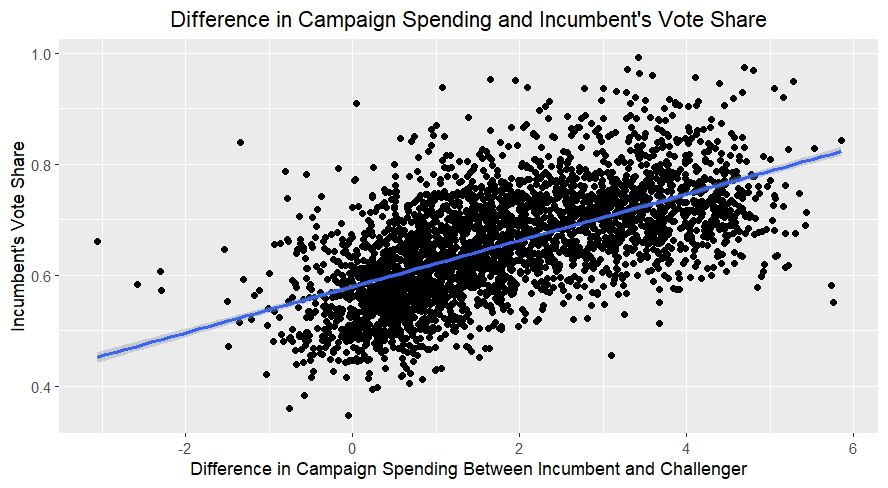
\includegraphics[width=0.88\textwidth]{Question_1_scatterplot.jpeg}
		\end{figure}
		
		\item Save the residuals of the model in a separate object.
		\lstinputlisting[language=R, firstline=54, lastline=55]{PS03_answersKC.R}
		
		\item Write the prediction equation.
	    
	    \noindent The numbers representing the slope and y-intercept are taken from the linear regression run in R.
		\noindent $$\hat{Y} = 0.04167X + 0.57903 $$
		\noindent In the equation, Y-hat represents the predicted value of the incumbent's vote share, and X represents the difference in campaign spending between incumbent and challenger.
		
	\end{enumerate}
	
\newpage

\section*{Question 2}
\noindent We are interested in knowing how the difference between incumbent and challenger's spending and the vote share of the presidential candidate of the incumbent's party are related.
	\begin{enumerate}
		\item Run a regression where the outcome variable is \texttt{presvote} and the explanatory variable is \texttt{difflog}.
		\lstinputlisting[language=R, firstline=64, lastline=64]{PS03_answersKC.R}

		\begin{verbatim}
Call:
lm(formula = presvote ~ difflog, data = inc.sub)

Coefficients:
(Intercept)      difflog  
    0.50758      0.02384  
		\end{verbatim}
		\item Make a scatterplot of the two variables and add the regression line.
		\lstinputlisting[language=R, firstline=67, lastline=73]{PS03_answersKC.R}

		\begin{figure} [h]
			\centering
			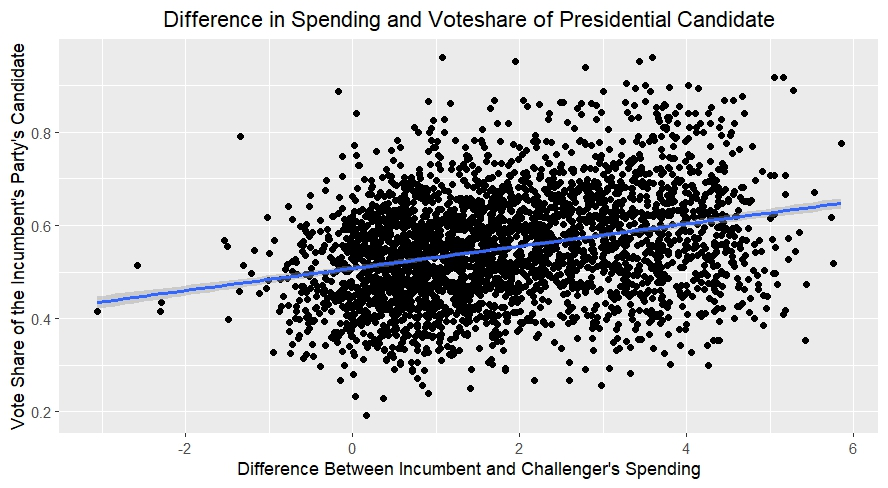
\includegraphics[width=0.88\textwidth]{Question_2_scatterplot.jpeg}
		\end{figure}
	    \newpage
		\item Save the residuals of the model in a separate object.
		\lstinputlisting[language=R, firstline=76, lastline=77]{PS03_answersKC.R}
		
		
		\item Write the prediction equation.
		
		\noindent The numbers representing the slope and y-intercept are taken from the linear regression run in R.
		
		$$ \hat{Y} = .02384X + 0.50758 $$
		
		\noindent In the equation, Y-hat represents the predicted value of vote share of the presidential candidate of the incumbent's party, and X represents the difference between incumbent and challenger's spending.
		
	\end{enumerate}
	\vspace{.25cm}
\section*{Question 3}

\noindent We are interested in knowing how the vote share of the presidential candidate of the incumbent's party is associated with the incumbent's electoral success.
	\vspace{.25cm}
	\begin{enumerate}
		\item Run a regression where the outcome variable is \texttt{voteshare} and the explanatory variable is \texttt{presvote}.
        \lstinputlisting[language=R, firstline=87, lastline=87]{PS03_answersKC.R}
\begin{verbatim}
Call:
lm(formula = voteshare ~ presvote, data = inc.sub)

Coefficients:
(Intercept)     presvote  
     0.4413       0.3880  
\end{verbatim}

		\item Make a scatterplot of the two variables and add the regression line. 
        \lstinputlisting[language=R, firstline=90, lastline=96]{PS03_answersKC.R}

\begin{figure} [h]
    \centering
	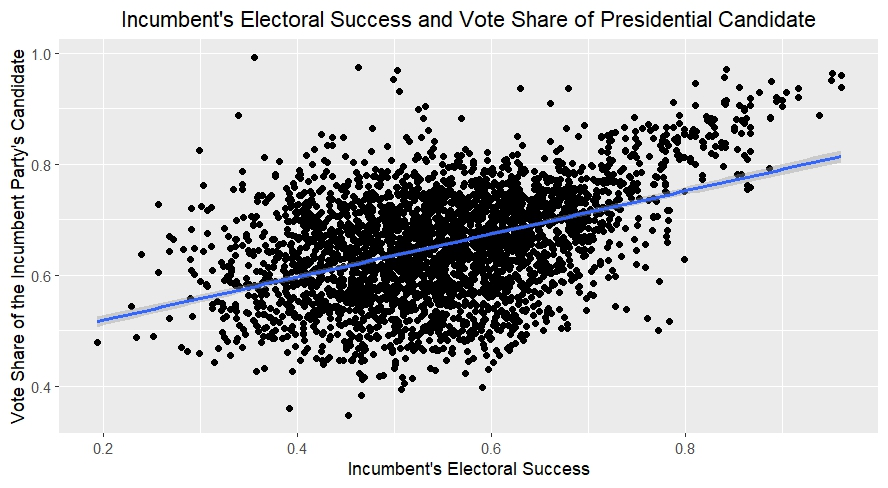
\includegraphics[width=0.88\textwidth]{Question_3_scatterplot.jpeg}
\end{figure}

		\item Write the prediction equation.
	
	\noindent The numbers representing the slope and y-intercept are taken from the linear regression run in R.
	
		\noindent $$ \hat{Y} = 0.3880X + 0.4413 $$
		
		\noindent In the equation, Y-hat represents the predicted value of the vote share of the presidential candidate of the incumbent party, and X represents the incumbent's electoral success.
		
	\end{enumerate}
	\vspace{.25cm}
\section*{Question 4}
\noindent The residuals from part (a) tell us how much of the variation in \texttt{voteshare} is $not$ explained by the difference in spending between incumbent and challenger. The residuals in part (b) tell us how much of the variation in \texttt{presvote} is $not$ explained by the difference in spending between incumbent and challenger in the district.
	\begin{enumerate}
		\item Run a regression where the outcome variable is the residuals from Question 1 and the explanatory variable is the residuals from Question 2.
		\lstinputlisting[language=R, firstline=104, lastline=104]{PS03_answersKC.R}
		\newpage
		\begin{verbatim}
Call:
lm(formula = residuals1 ~ residuals2, data = inc.sub)

Coefficients:
(Intercept)                residuals2  
-0.000000000000000005934   0.256877012700097440145 
		\end{verbatim}
		
		\item Make a scatterplot of the two residuals and add the regression line.
		\lstinputlisting[language=R, firstline=107, lastline=113]{PS03_answersKC.R}
		\begin{figure} [h]
			\centering
			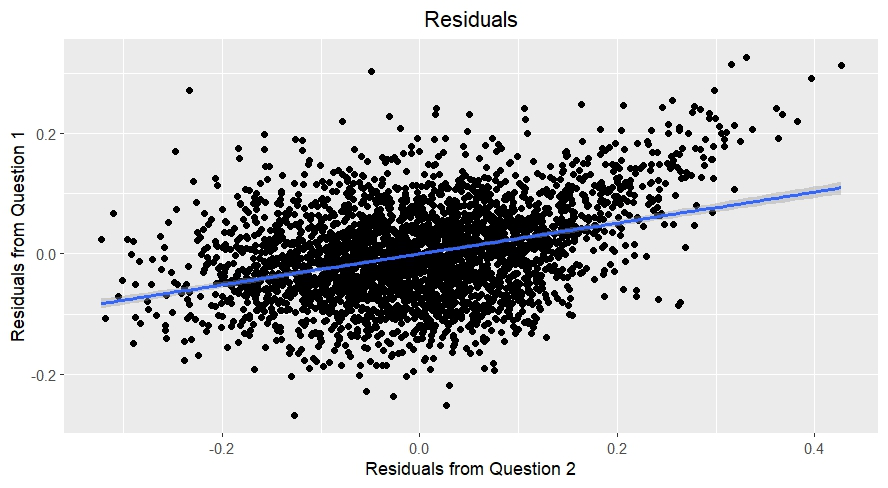
\includegraphics[width=0.88\textwidth]{Question_4_scatterplot.jpeg}
		\end{figure}
		
		\item Write the prediction equation.
		
		\noindent $$ \hat{Y} = 0.256877012700097440145X - 0.000000000000000005934 $$ 
		
		\noindent In the equation, Y-hat represents the predicted value of the variation in voteshare that is not explained by the difference in spending between incumbent and challenger and X represents the variation in presvote not explained by the difference in spending between incumbent and challenger in the district. In other words, this regression shows the linear impact of presvote on voteshare if the linear impact of difflog is removed.
	\end{enumerate}
	
	\newpage	

\section*{Question 5}
\noindent What if the incumbent's vote share is affected by both the president's popularity and the difference in spending between incumbent and challenger? 
	\begin{enumerate}
		\item Run a regression where the outcome variable is the incumbent's \texttt{voteshare} and the explanatory variables are \texttt{difflog} and \texttt{presvote}.
		\lstinputlisting[language=R, firstline=128, lastline=128]{PS03_answersKC.R}
		\begin{verbatim}
Call:
lm(formula = voteshare ~ difflog + presvote, data = inc.sub)

Coefficients:
(Intercept)      difflog     presvote  
    0.44864      0.03554      0.25688 
		\end{verbatim}
		\item Write the prediction equation.
		
		\noindent The numbers representing the slope and y-intercept are taken from the linear regression run in R.
		
		\noindent $$\hat{Y} = 0.44864 + 0.03554X_{1} + 0.25688X_{2} $$
	
    	\noindent In the prediction equation, Y-hat represents the predicted value of the incumbent's vote share, X1 represents the difference in spending between incumbent and challenger, and X2 represents the president's popularity.
	
		\vspace{.25cm}
		\item What is it in this output that is identical to the output in Question 4? Why do you think this is the case?
	
		\vspace{.25cm}
	
		\noindent The coefficient for presvote, 0.25688, is identical to the output in Question 4. The residuals from Question 1 represent the part of voteshare that cannot be linearly explained by difflog. The residuals from Question 2 represent the part of presvote that cannot be linearly explained by difflog. In Question 4, we are looking for a linear relationship between the residuals and we got the coefficient 0.25688, which represents the impact of presvote on vote share if you take out the impact of difflog. In Question 5, 0.25688 represents the impact of presvote on voteshare, linearly adjusting for difflog, assuming that difflog and presvote are uncorrelated. Therefore, since in both cases the coefficient represents the linear impact of presvote on voteshare without the impact of difflog, the coefficients are the same. Following this logic, if I were to do a summary of the linear regressions, it would show that the standard errors of the coefficients are also the same.
		
		
		
	\end{enumerate}




\end{document}
